% content/talk.tex
% Main talk content: frames only.

% Optional: outline slide each section
\AtBeginSection[]{
  \begin{frame}{Outline}
    \tableofcontents[currentsection]
  \end{frame}
}

\begin{frame}{Outline}
  \tableofcontents
\end{frame}

\section{Motivation}

\begin{frame}{Problem statement}
  \begin{itemize}
    \item You have a 15-minute talk with optional deep-dive backup.
    \item You want slide numbers like \texttt{3/12} that ignore backups.
    \item You want a consistent theme with minimal preamble glue.
  \end{itemize}

  \vspace{0.6em}
  \begin{block}{Goal}
    Keep the audience-oriented count stable while still shipping detail slides.
  \end{block}
\end{frame}

\begin{frame}{Two-column slide}
  \begin{columns}[T,onlytextwidth]
    \column{0.52\textwidth}
      \begin{itemize}
        \item Left column: bullets
        \item A key point
        \item Another key point
      \end{itemize}
      \begin{alertblock}{Risk}
        Too much text per slide.
      \end{alertblock}

    \column{0.48\textwidth}
      \begin{exampleblock}{Mitigation}
        Use figures, progressive disclosure, and backups.
      \end{exampleblock}
      \begin{itemize}
        \item Keep slides visual
        \item Put derivations in backup
      \end{itemize}
  \end{columns}
\end{frame}

\section{Approach}

\begin{frame}{A slide with a figure}
  \begin{figure}
    \centering
    % Put any placeholder image at figs/example.png
    
\includegraphics[width=0.85\linewidth]{example.png}
    \caption{Example figure (replace with your real plot).}
  \end{figure}
\end{frame}

\begin{frame}{Math / equations}
  \begin{block}{Model}
    \[
      y = f_\theta(x) + \epsilon,\qquad \epsilon \sim \mathcal{N}(0,\sigma^2)
    \]
  \end{block}

  \begin{itemize}
    \item Emphasize assumptions and what is measured.
    \item Move lengthy derivations to backup.
  \end{itemize}
\end{frame}

\begin{frame}{Blocks and takeaways}
  \begin{block}{Key result}
    We reduce confusion by separating \emph{main} vs \emph{backup} frames.
  \end{block}

  \begin{alertblock}{Common pitfall}
    Counting backup frames in the total makes the talk feel longer than it is.
  \end{alertblock}

  \begin{exampleblock}{Practical pattern}
    Main narrative: 10--15 frames. Backup: as many as needed.
  \end{exampleblock}
\end{frame}

\begin{frame}{Table slide}
  \centering
  \begin{tabular}{lccc}
    \hline
    Method & Metric A $\uparrow$ & Metric B $\downarrow$ & Notes \\
    \hline
    Baseline & 0.72 & 1.31 & simple \\
    Ours     & 0.81 & 1.02 & best \\
    Ablation & 0.78 & 1.12 & remove X \\
    \hline
  \end{tabular}

  \vspace{0.8em}
  \begin{itemize}
    \item Keep tables sparse.
    \item Highlight one row/column in narration, not color.
  \end{itemize}
\end{frame}

\begin{frame}[fragile]{Code slide (verbatim)}
  % Beamer + verbatim: mark the frame as fragile
  \begin{center}
    \textbf{Minimal example snippet}
  \end{center}

  \vspace{0.5em}
  \begin{verbatim}
# python
import numpy as np

x = np.linspace(0, 1, 1000)
y = np.sin(2*np.pi*5*x)
print(y.mean())
  \end{verbatim}
\end{frame}

\begin{frame}{Diagram slide (TikZ)}
  \centering
  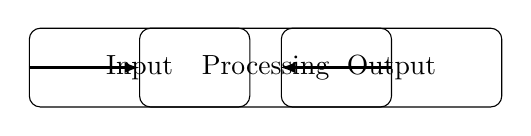
\begin{tikzpicture}[node distance=1.6cm,>=latex]
    \node (a) [draw, rounded corners, minimum width=2.8cm, minimum height=1cm] {Input};
    \node (b) [draw, rounded corners, right of=a, minimum width=3.2cm, minimum height=1cm] {Processing};
    \node (c) [draw, rounded corners, right of=b, minimum width=2.8cm, minimum height=1cm] {Output};
    \draw[->, thick] (a) -- (b);
    \draw[->, thick] (b) -- (c);
  \end{tikzpicture}

  \vspace{0.8em}
  \begin{itemize}
    \item Use simple boxes/arrows in main talk.
    \item Put full architecture diagrams in backup.
  \end{itemize}
\end{frame}

\section{Results}

\begin{frame}{Results slide}
  \begin{itemize}
    \item Claim 1 with a number (or plot).
    \item Claim 2 with a comparison baseline.
    \item One sentence: why it matters.
  \end{itemize}

  \vspace{0.6em}
  \begin{block}{Takeaway}
    Your audience remembers \emph{one} takeaway per slide.
  \end{block}
\end{frame}

\section{Conclusion}

\begin{frame}{Summary}
  \begin{itemize}
    \item What you built / proved
    \item What you measured
    \item What changed vs baseline
    \item Next step
  \end{itemize}

  \vspace{0.6em}
  \begin{exampleblock}{Call to action}
    Put detailed evidence in backup slides; keep the narrative clean.
  \end{exampleblock}
\end{frame}

\begin{frame}{Q\&A}
  \centering
  \vfill
  {\Large Questions?}
  \vfill
  \begin{itemize}
    \item You can jump to backups as needed.
  \end{itemize}
\end{frame}
